%!TEX root = ../TTK4550-MHT.tex
\begin{figure}[H]
    \centering
    \textbf{Scenario 1 - Track performance}\par \medskip
    \begin{subfigure}{0.49\textwidth}
        \centering
        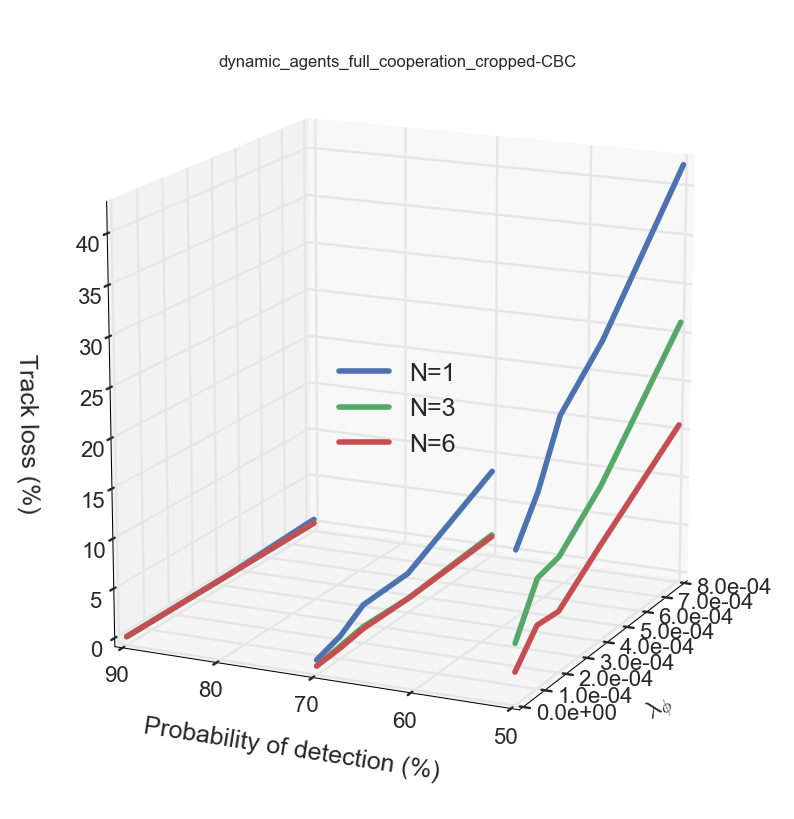
\includegraphics[width=\textwidth]{dynamic_agents_full_cooperation_cropped-CBC}
        \caption{CBC solver}
    \end{subfigure}
    \begin{subfigure}{0.49\textwidth}
        \centering
        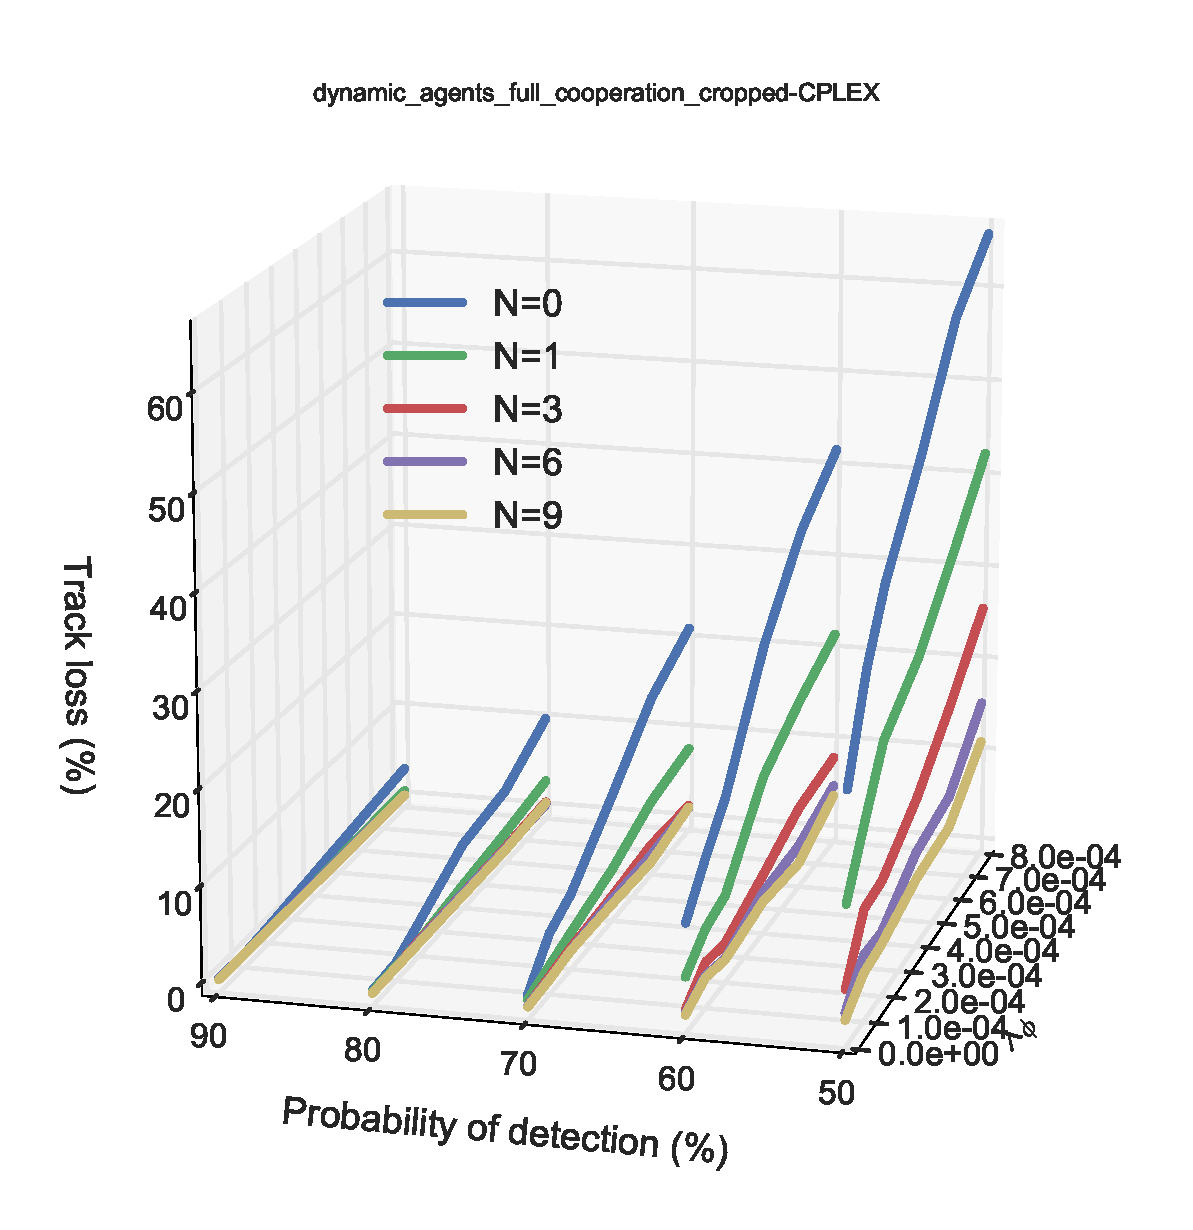
\includegraphics[width=\textwidth]{dynamic_agents_full_cooperation_cropped-CPLEX}
        \caption{CPLEX solver}
    \end{subfigure}
    \begin{subfigure}{0.49\textwidth}
        \centering
        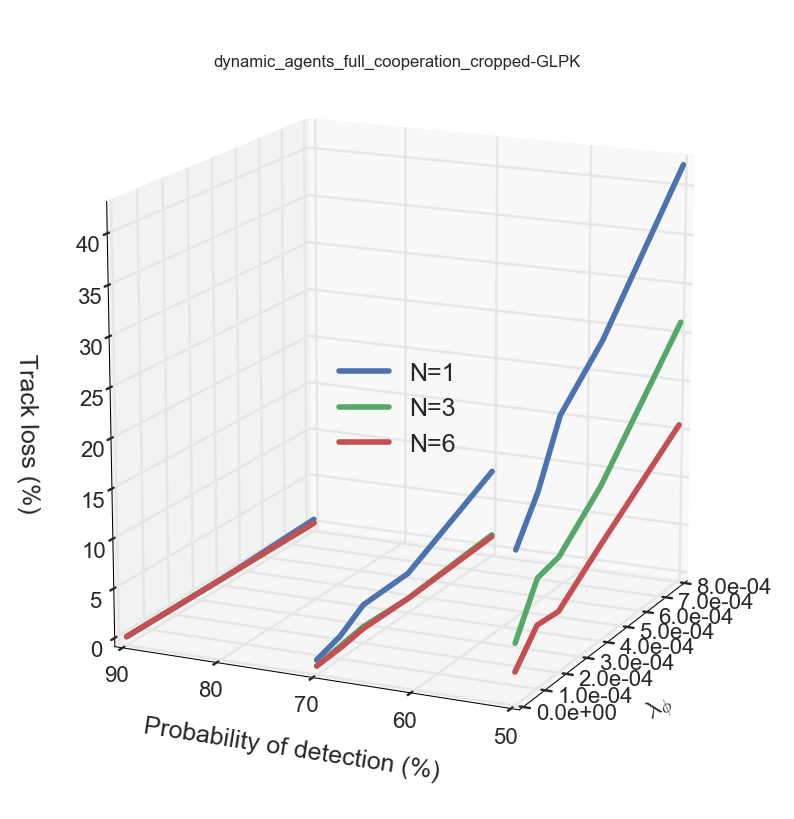
\includegraphics[width=\textwidth]{dynamic_agents_full_cooperation_cropped-GLPK}
        \caption{GLPK solver}
    \end{subfigure}
    \begin{subfigure}{0.49\textwidth}
        \centering
        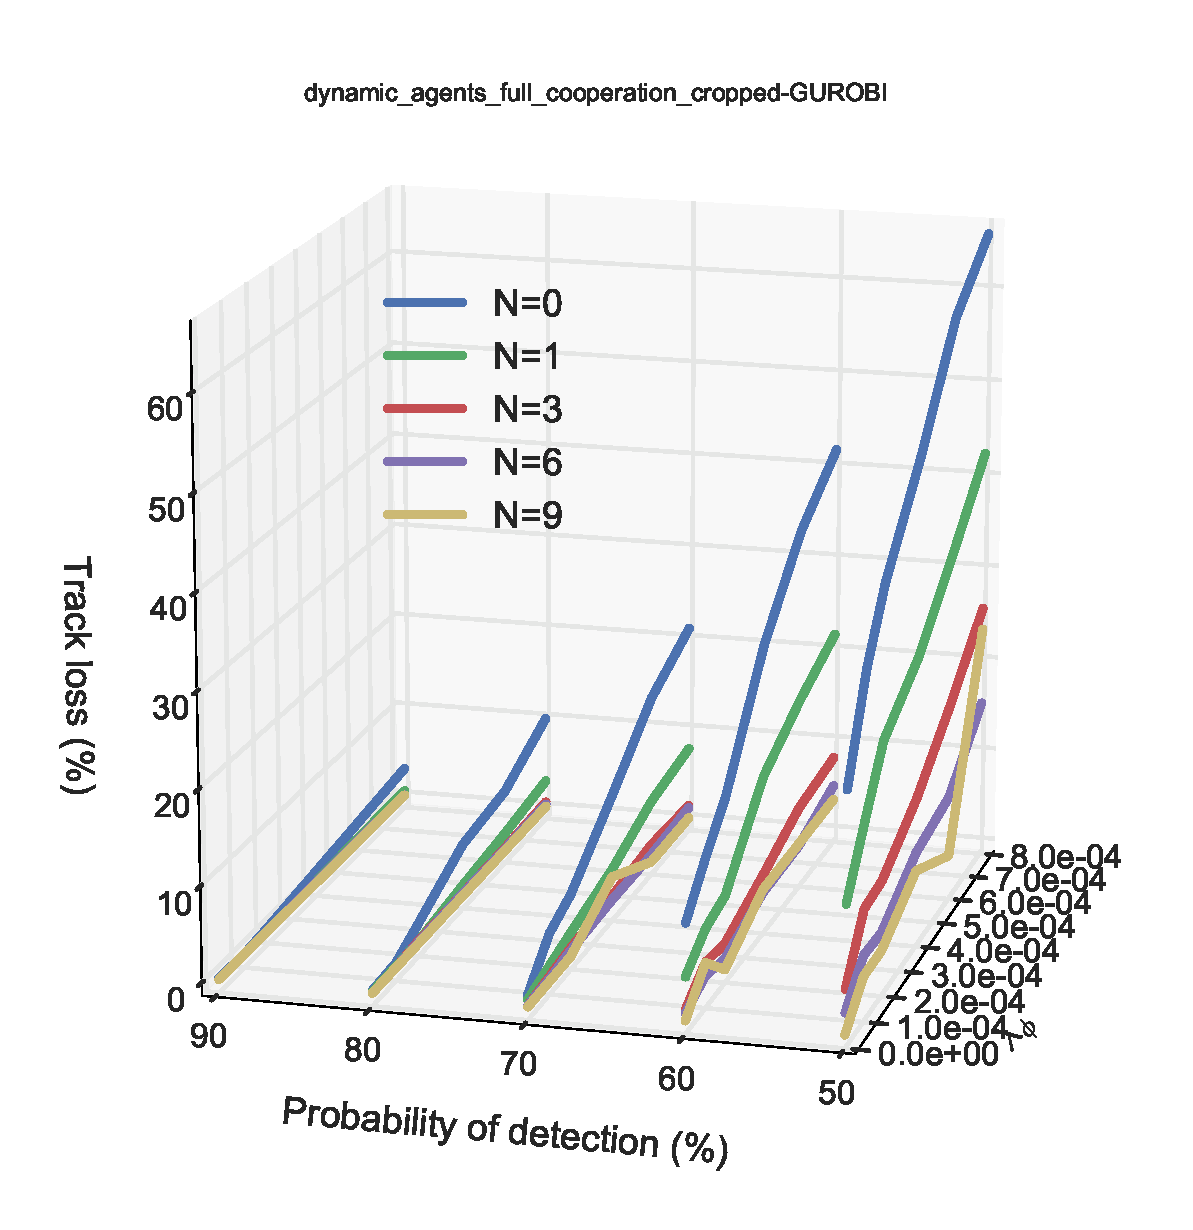
\includegraphics[width=\textwidth]{dynamic_agents_full_cooperation_cropped-GUROBI}
        \caption{GUROBI solver}
    \end{subfigure}
	\caption{Simulation results for all solvers in scenario 1}
    \label{fig:dynamic_agents_full_cooperation_cropped}
\end{figure}
\begin{figure}[H]
    \centering
    \textbf{Scenario 2 - Track performance}\par \medskip
    \begin{subfigure}{0.49\textwidth}
        \centering
        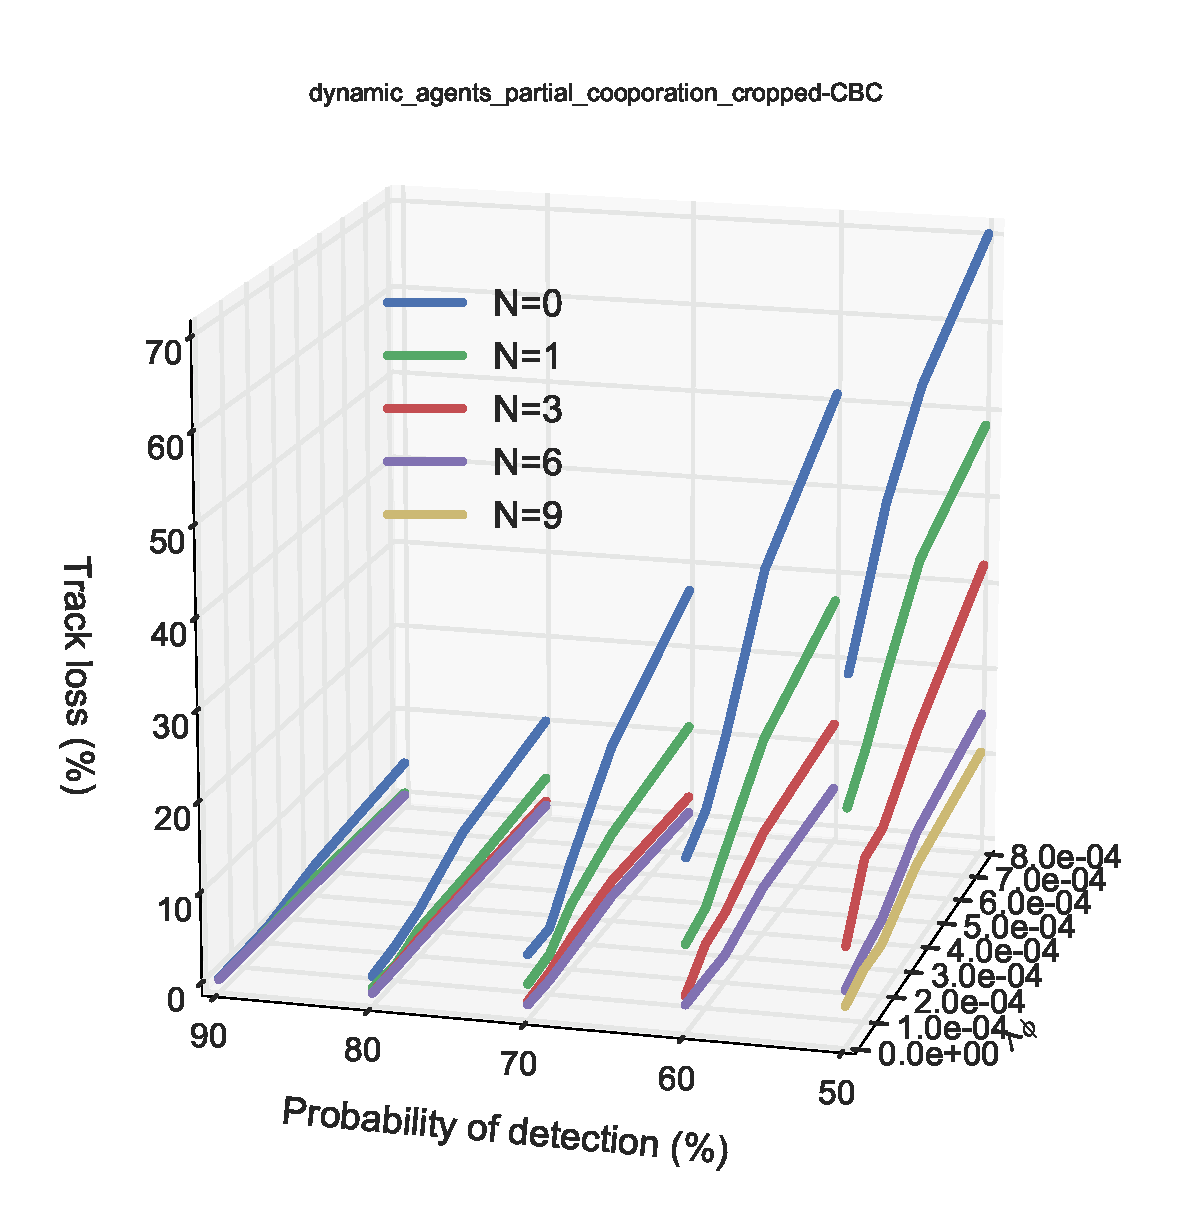
\includegraphics[width=\textwidth]{dynamic_agents_partial_cooporation_cropped-CBC}
        \caption{CBC solver}
    \end{subfigure}
    \begin{subfigure}{0.49\textwidth}
        \centering
        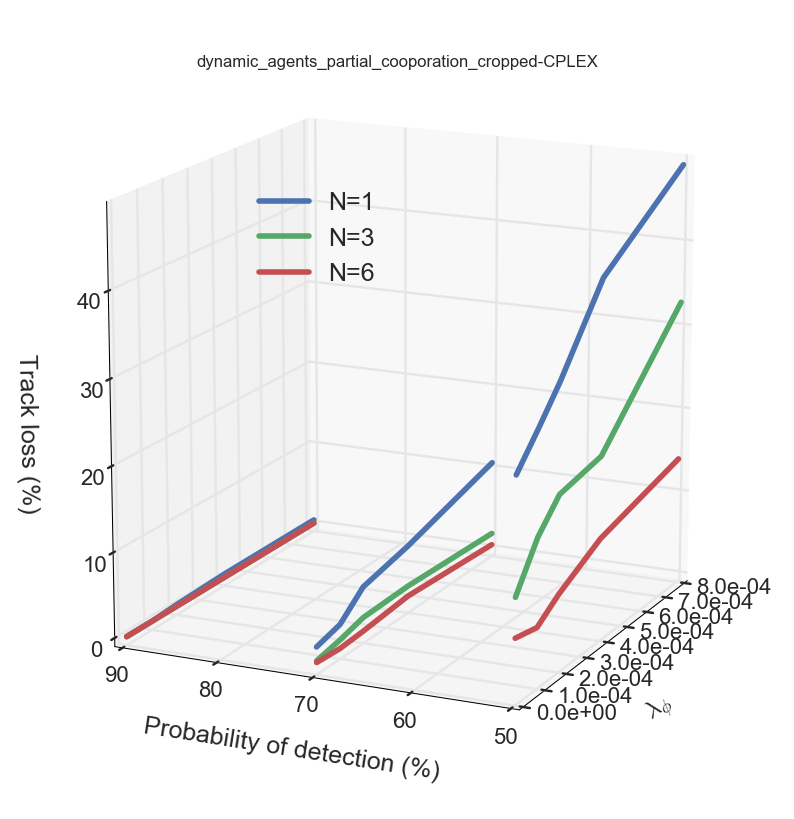
\includegraphics[width=\textwidth]{dynamic_agents_partial_cooporation_cropped-CPLEX}
        \caption{CPLEX solver}
    \end{subfigure}
    \begin{subfigure}{0.49\textwidth}
        \centering
        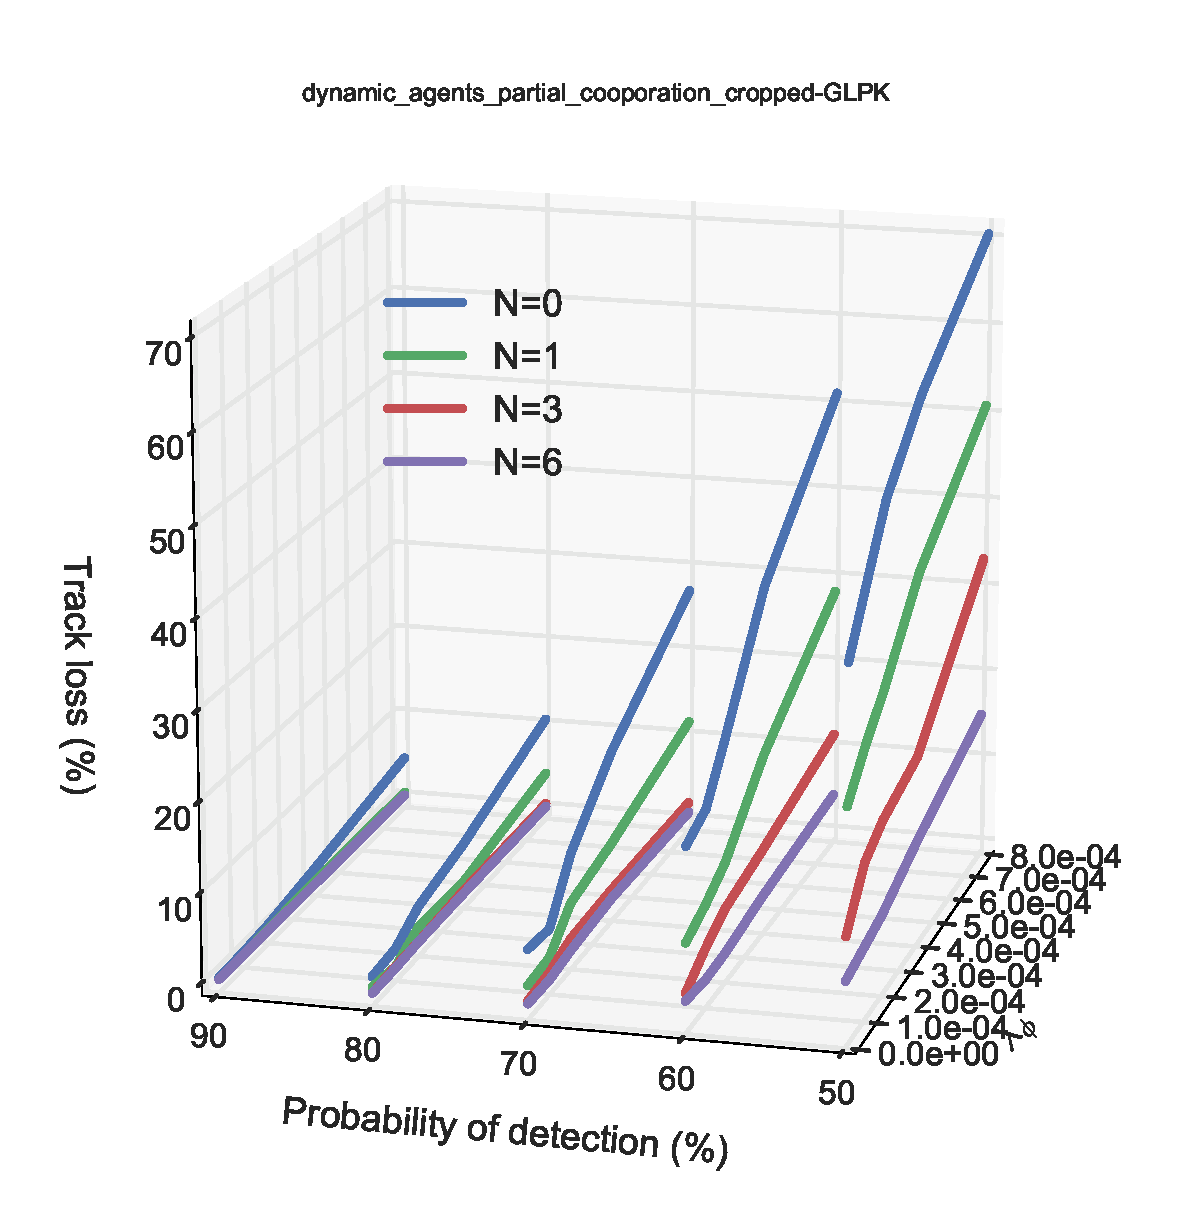
\includegraphics[width=\textwidth]{dynamic_agents_partial_cooporation_cropped-GLPK}
        \caption{GLPK solver}
    \end{subfigure}
    \begin{subfigure}{0.49\textwidth}
        \centering
        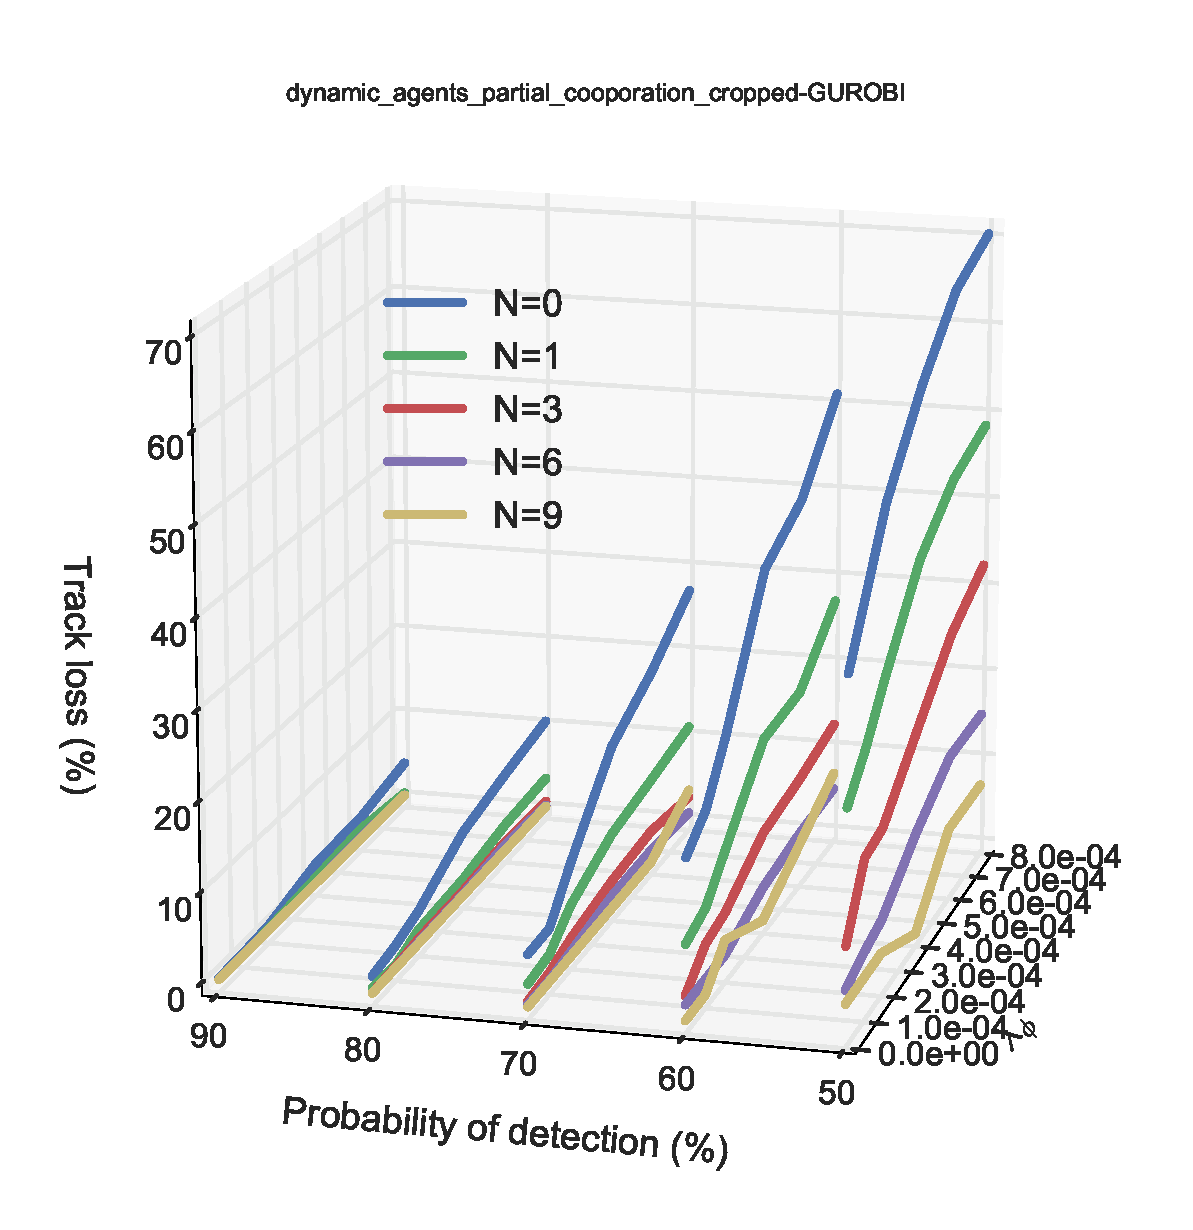
\includegraphics[width=\textwidth]{dynamic_agents_partial_cooporation_cropped-GUROBI}
        \caption{GUROBI solver}
    \end{subfigure}
    \caption{Simulation results for all solvers in scenario 2}
	\label{fig:dynamic_agents_partial_cooperation_cropped}
\end{figure}
\begin{figure}[H]
    \centering
    \textbf{Scenario3 - Track performance}\par \medskip
    \begin{subfigure}{0.49\textwidth}
        \centering
        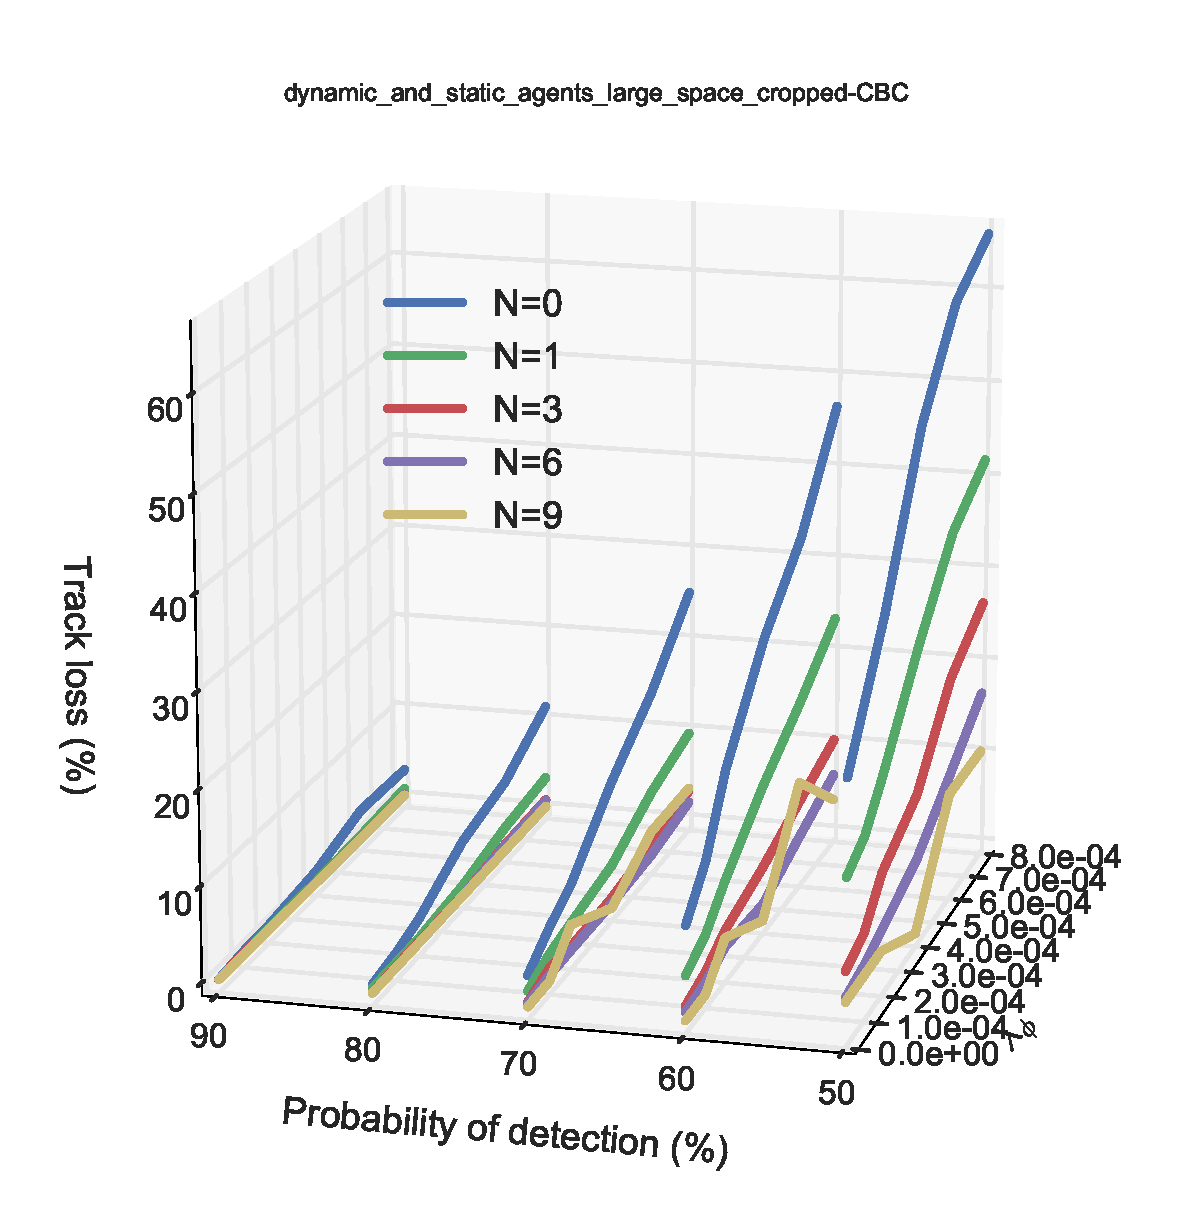
\includegraphics[width=\textwidth]{dynamic_and_static_agents_large_space_cropped-CBC}
        \caption{CBC solver}
    \end{subfigure}
    \begin{subfigure}{0.49\textwidth}
        \centering
        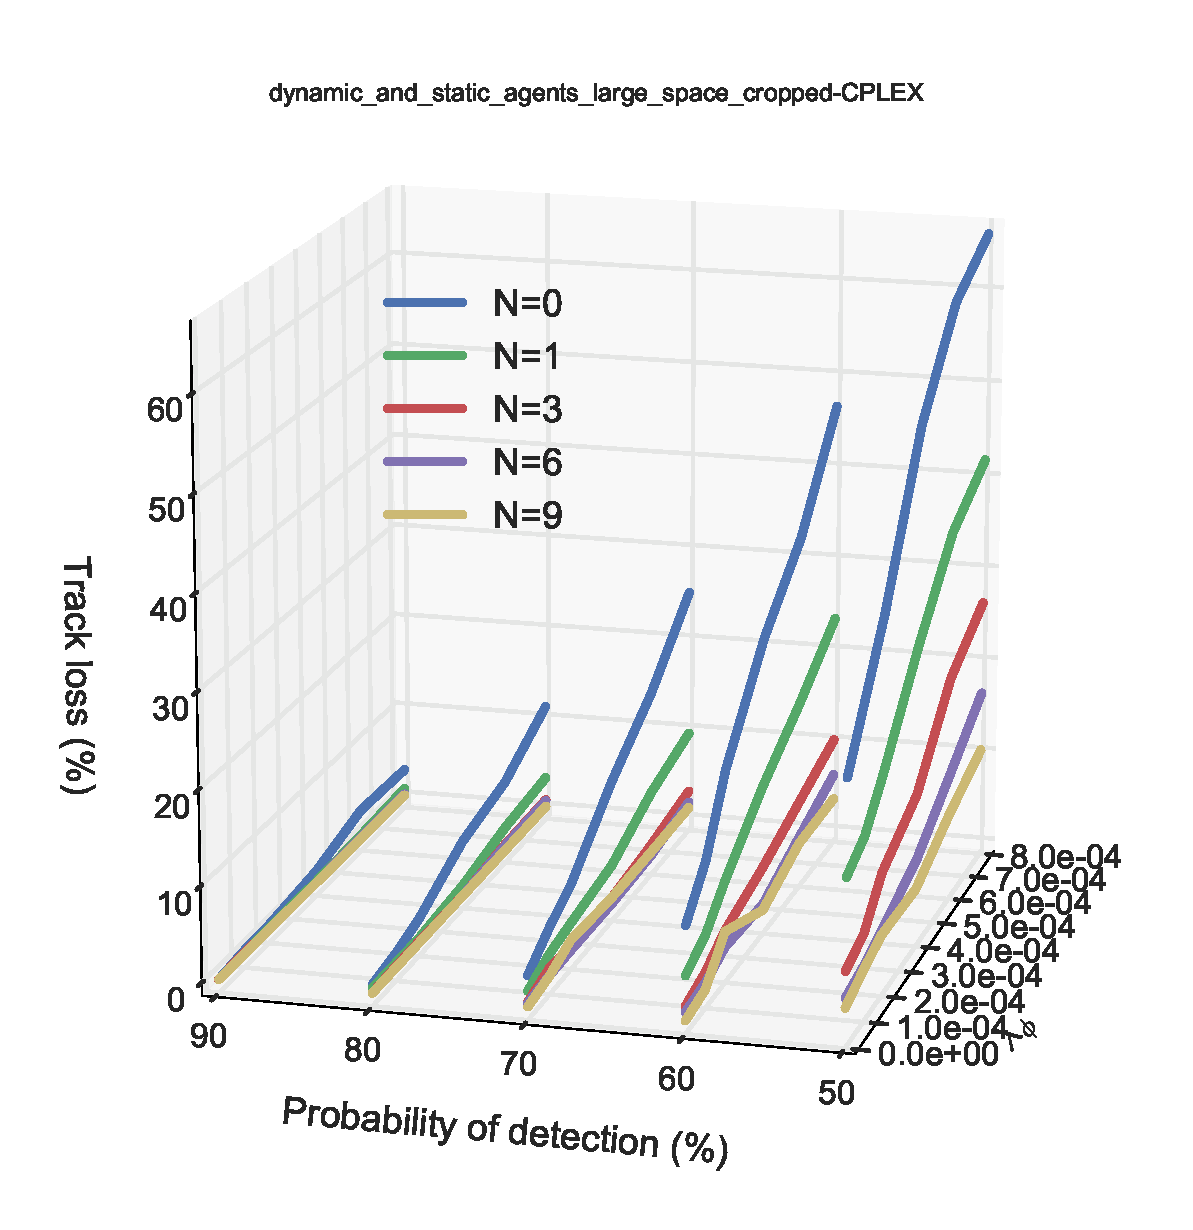
\includegraphics[width=\textwidth]{dynamic_and_static_agents_large_space_cropped-CPLEX}
        \caption{CPLEX solver}
    \end{subfigure}
    \begin{subfigure}{0.49\textwidth}
        \centering
        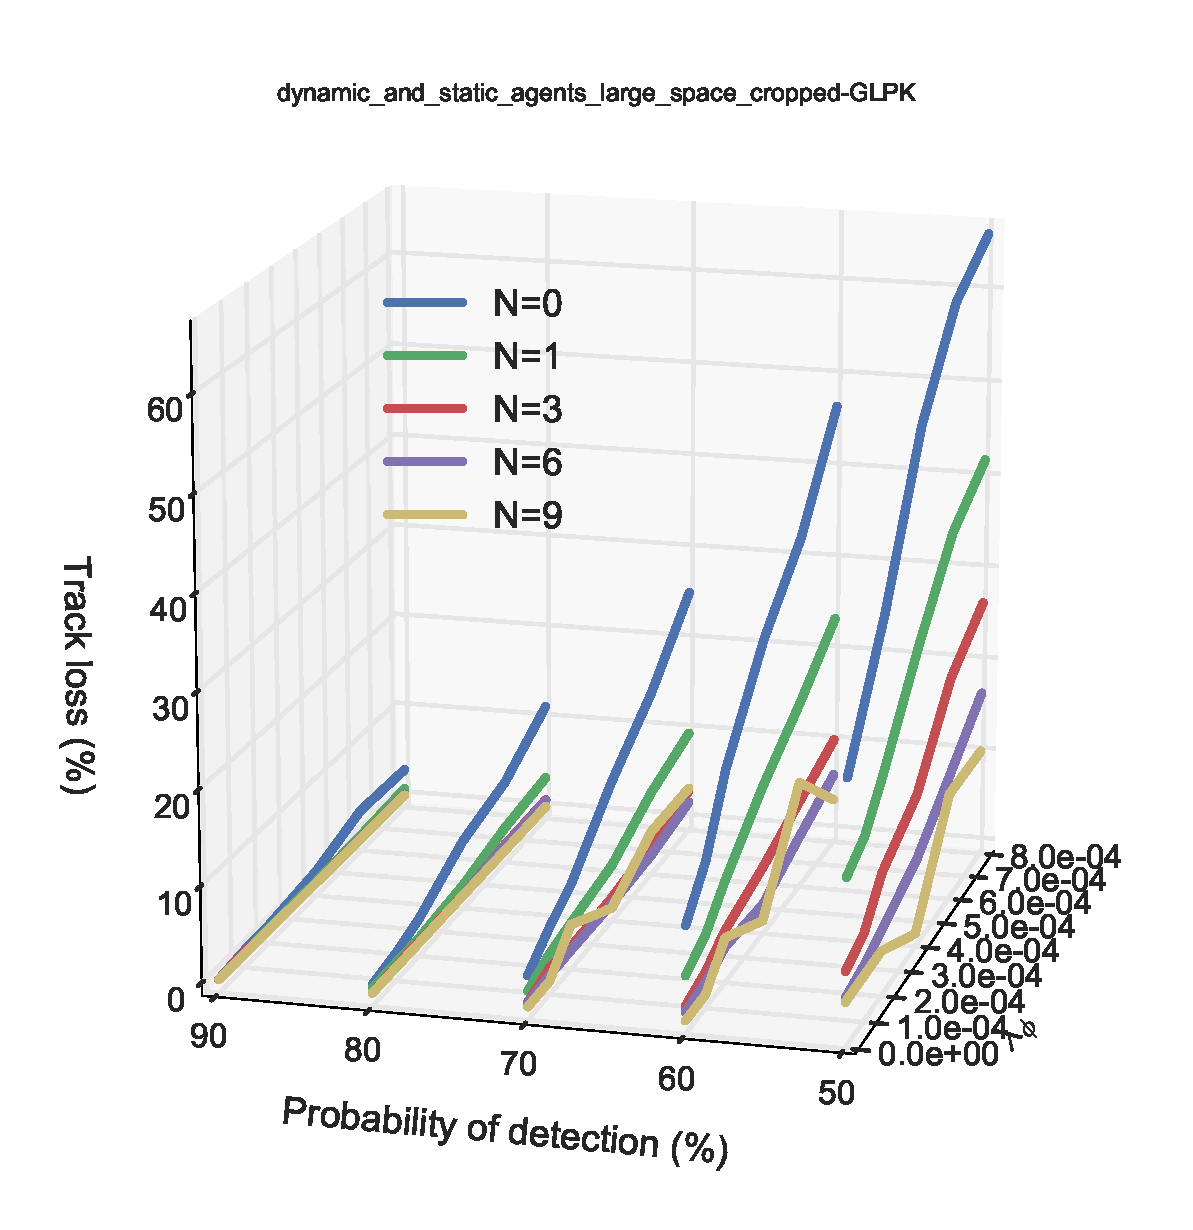
\includegraphics[width=\textwidth]{dynamic_and_static_agents_large_space_cropped-GLPK}
        \caption{GLPK solver}
    \end{subfigure}
    \begin{subfigure}{0.49\textwidth}
        \centering
        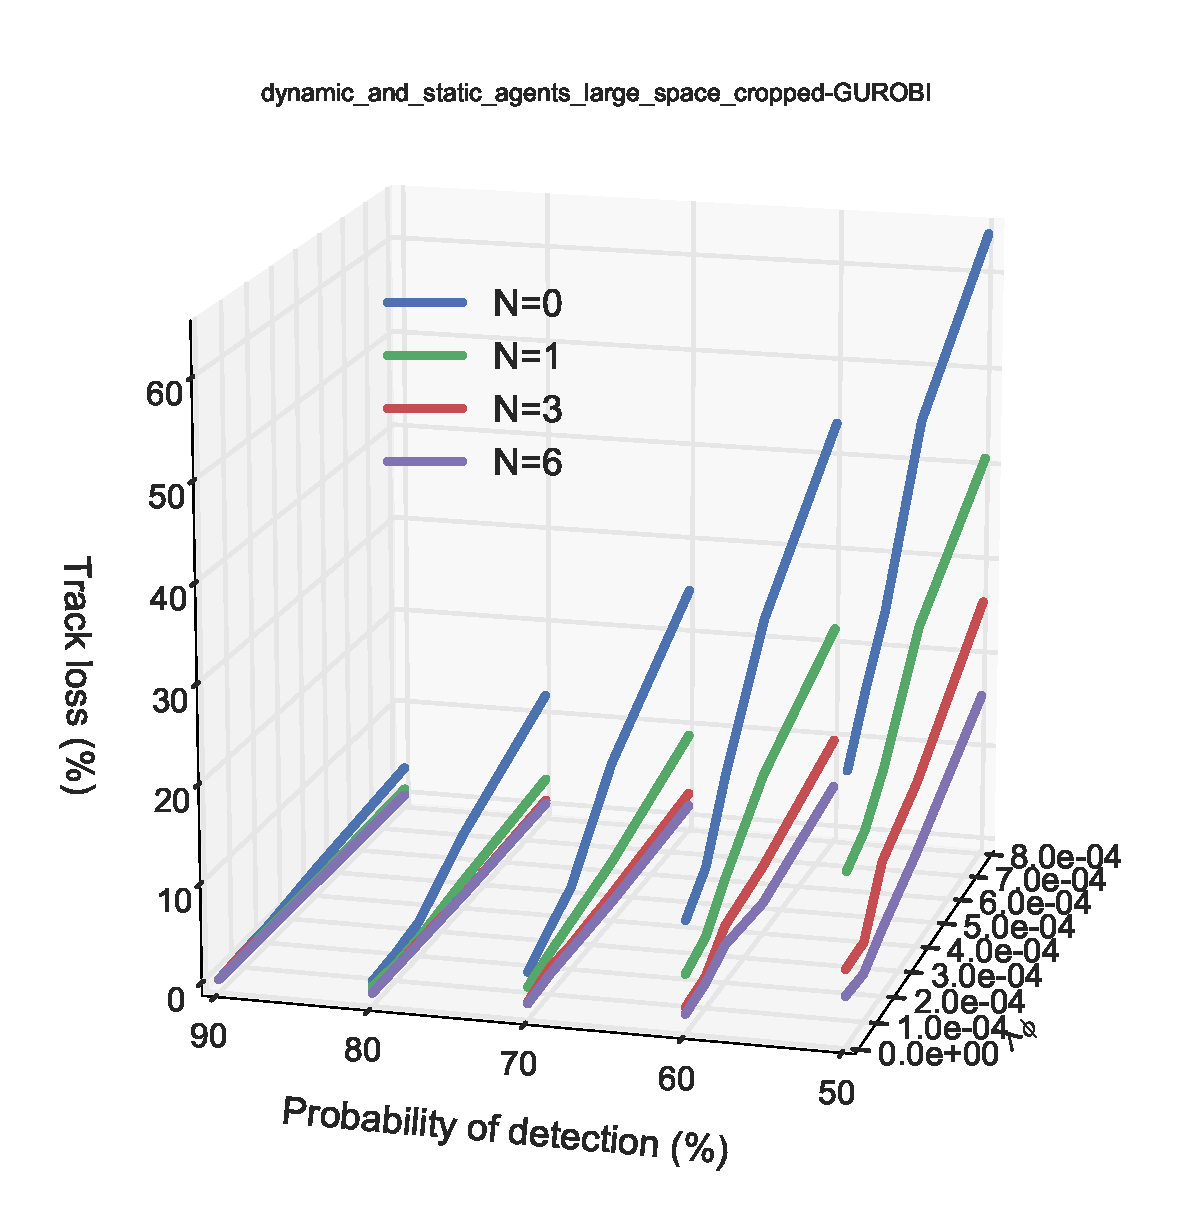
\includegraphics[width=\textwidth]{dynamic_and_static_agents_large_space_cropped-GUROBI}
        \caption{GUROBI solver}
    \end{subfigure}
    \caption{Simulation results for all solvers in scenario 3}
	\label{fig:dynamic_and_static_agents_large_space_cropped}
\end{figure}
\begin{figure}[H]
    \centering
    \textbf{Scenario 4 - Track performance}\par \medskip
    \begin{subfigure}{0.49\textwidth}
        \centering
        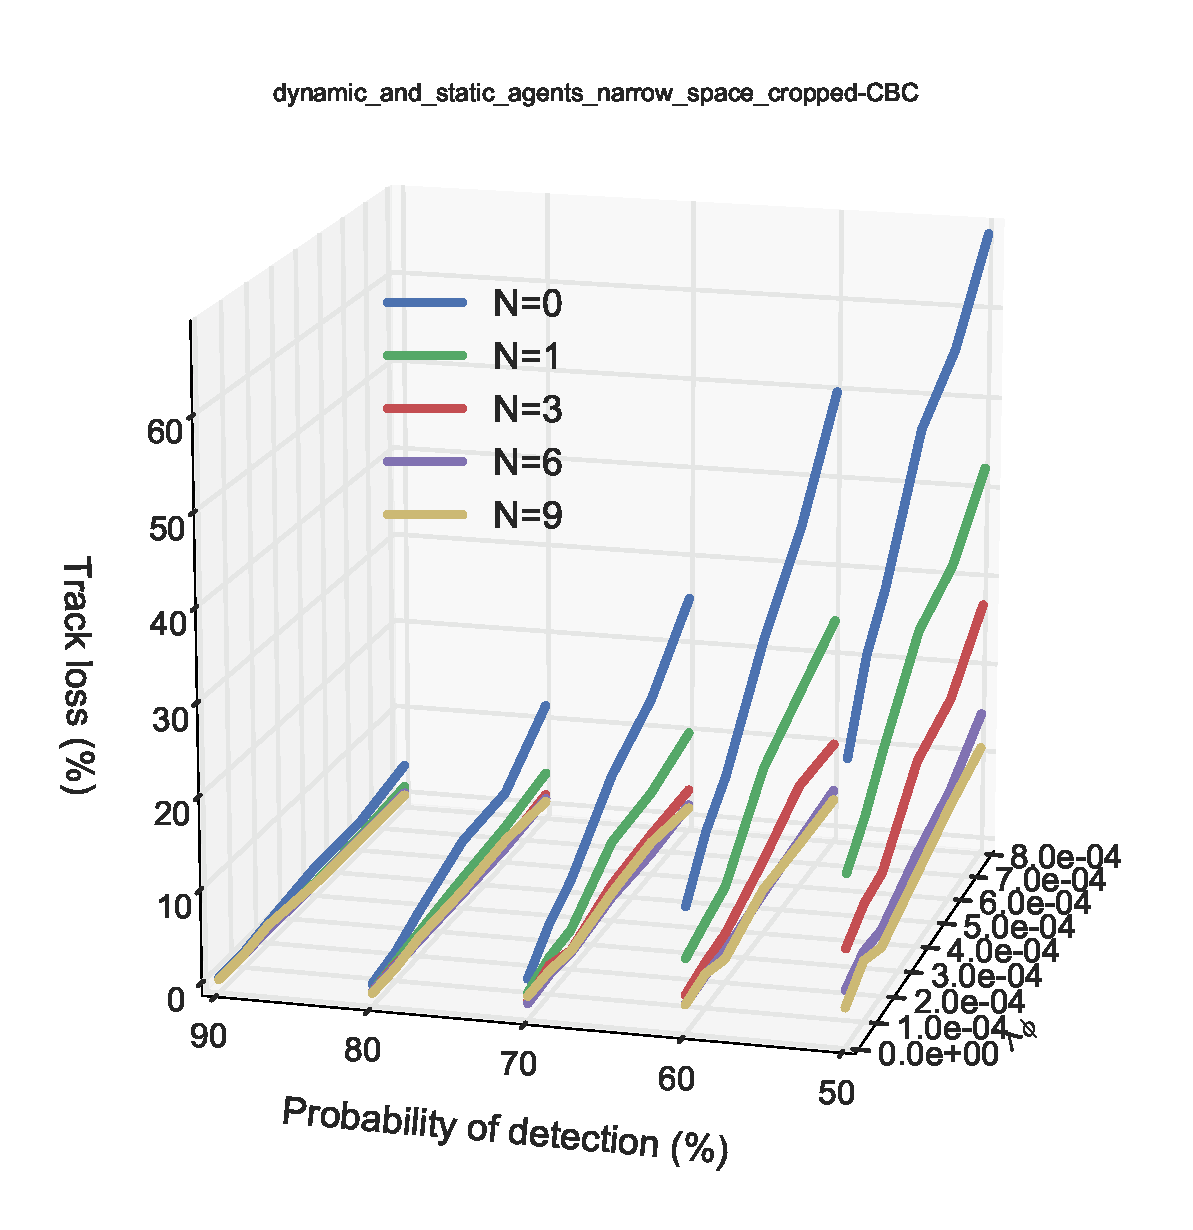
\includegraphics[width=\textwidth]{dynamic_and_static_agents_narrow_space_cropped-CBC}
        \caption{CBC solver}
    \end{subfigure}
    \begin{subfigure}{0.49\textwidth}
        \centering
        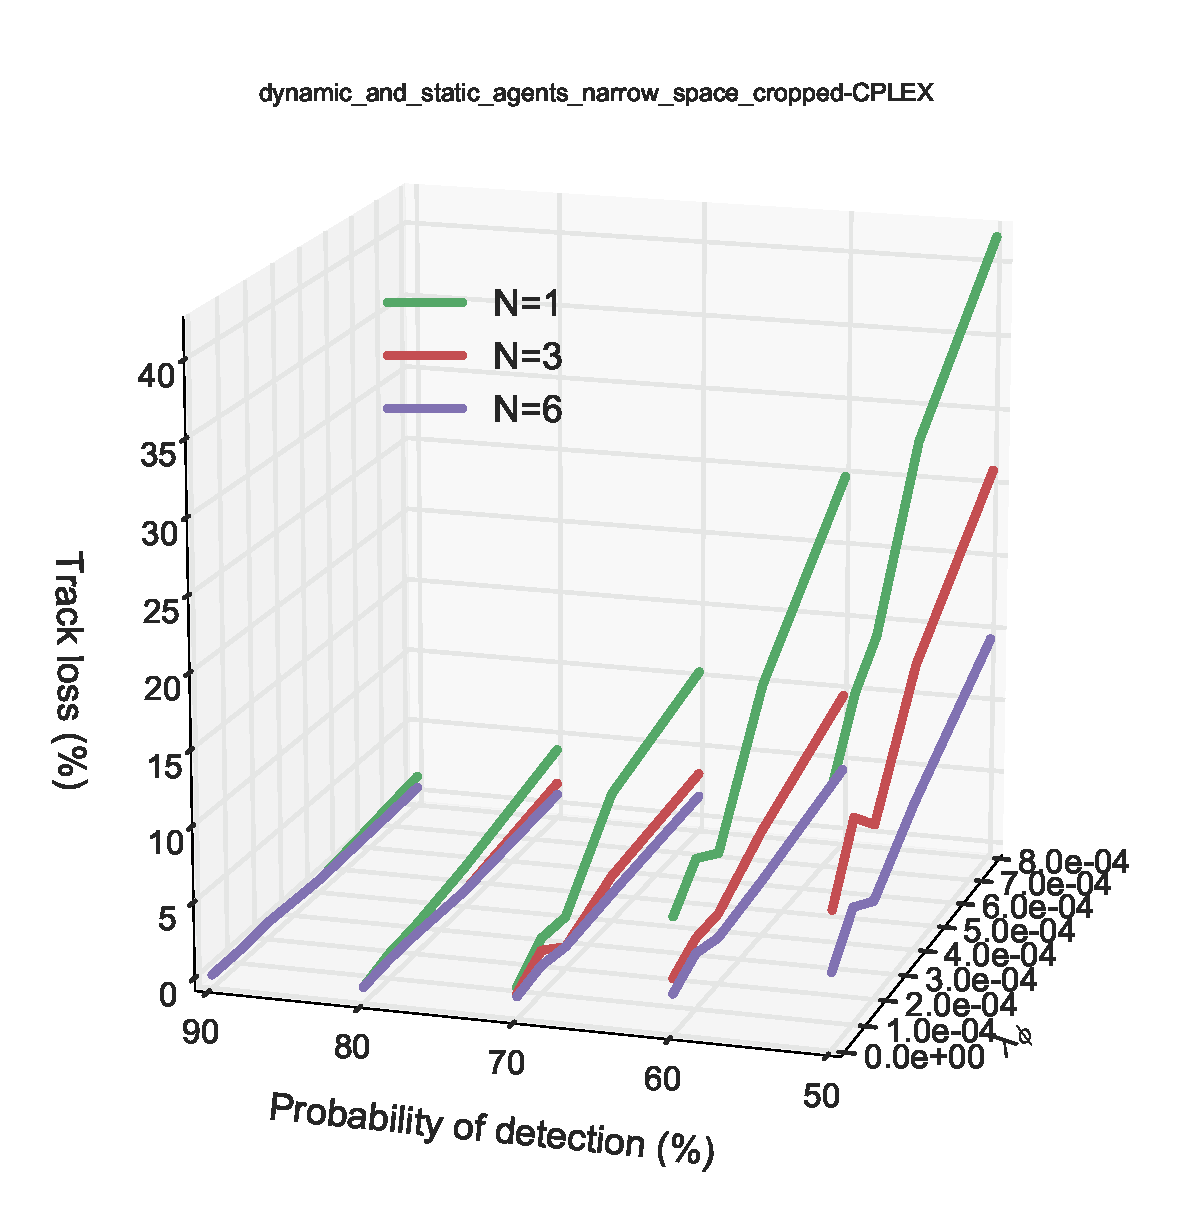
\includegraphics[width=\textwidth]{dynamic_and_static_agents_narrow_space_cropped-CPLEX}
        \caption{CPLEX solver}
    \end{subfigure}
    \begin{subfigure}{0.49\textwidth}
        \centering
        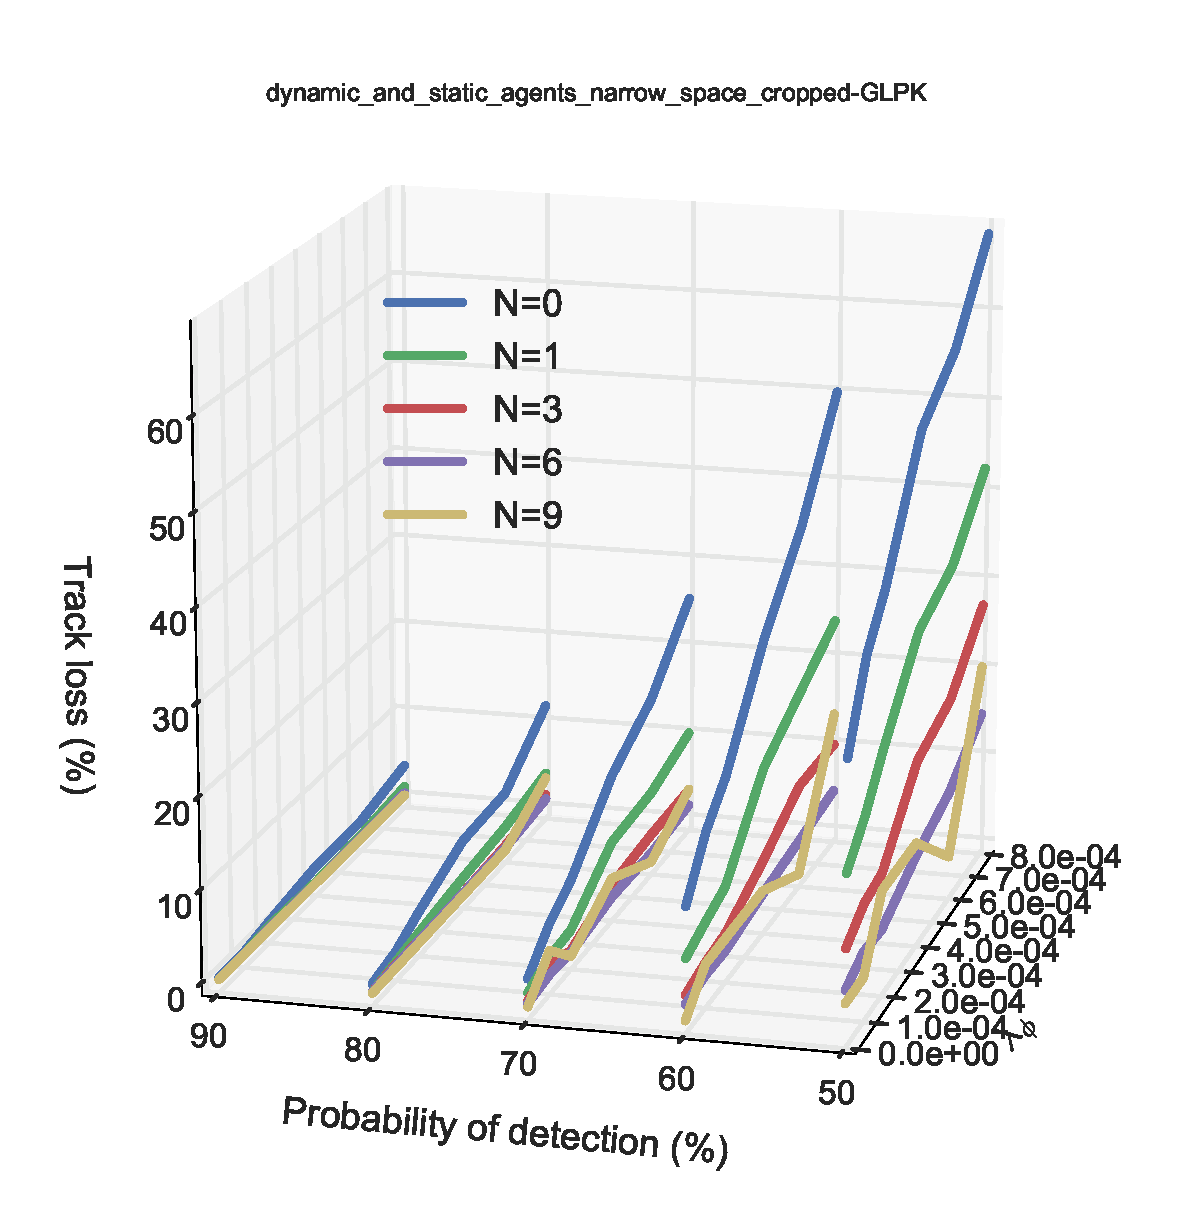
\includegraphics[width=\textwidth]{dynamic_and_static_agents_narrow_space_cropped-GLPK}
        \caption{GLPK solver}
    \end{subfigure}
    \begin{subfigure}{0.49\textwidth}
        \centering
        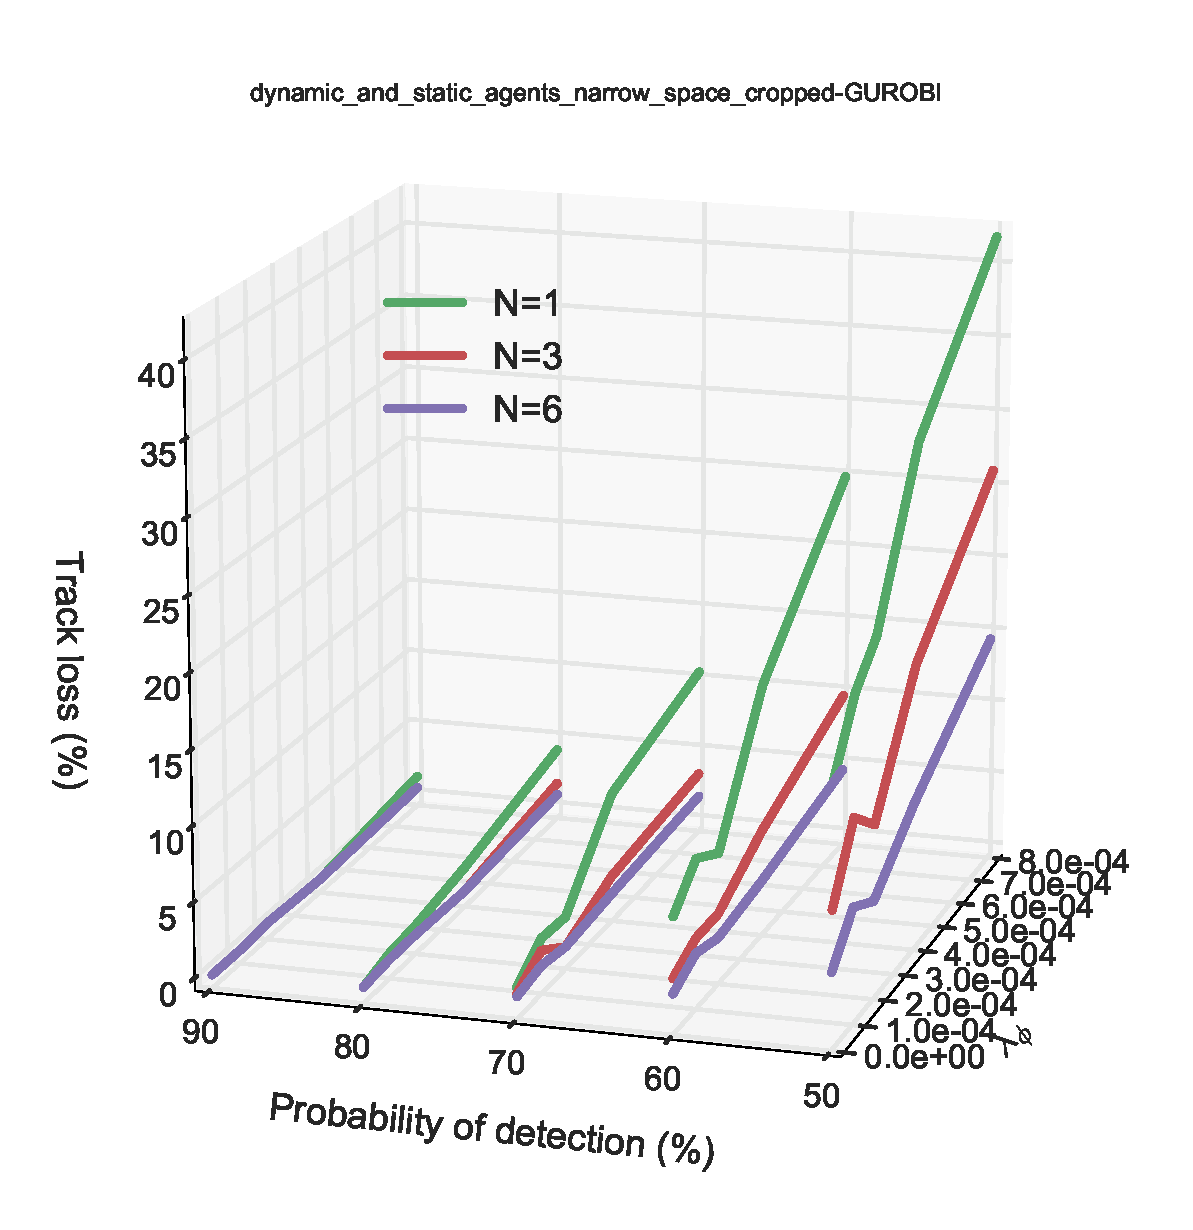
\includegraphics[width=\textwidth]{dynamic_and_static_agents_narrow_space_cropped-GUROBI}
        \caption{GUROBI solver}
    \end{subfigure}
    \caption{Simulation results for all solvers in scenario 4}
	\label{fig:dynamic_and_static_agents_narrow_space_cropped}
\end{figure}
\begin{figure}[H]
    \centering
    \textbf{Scenario 5 - Track performance}\par \medskip
    \begin{subfigure}{0.49\textwidth}
        \centering
        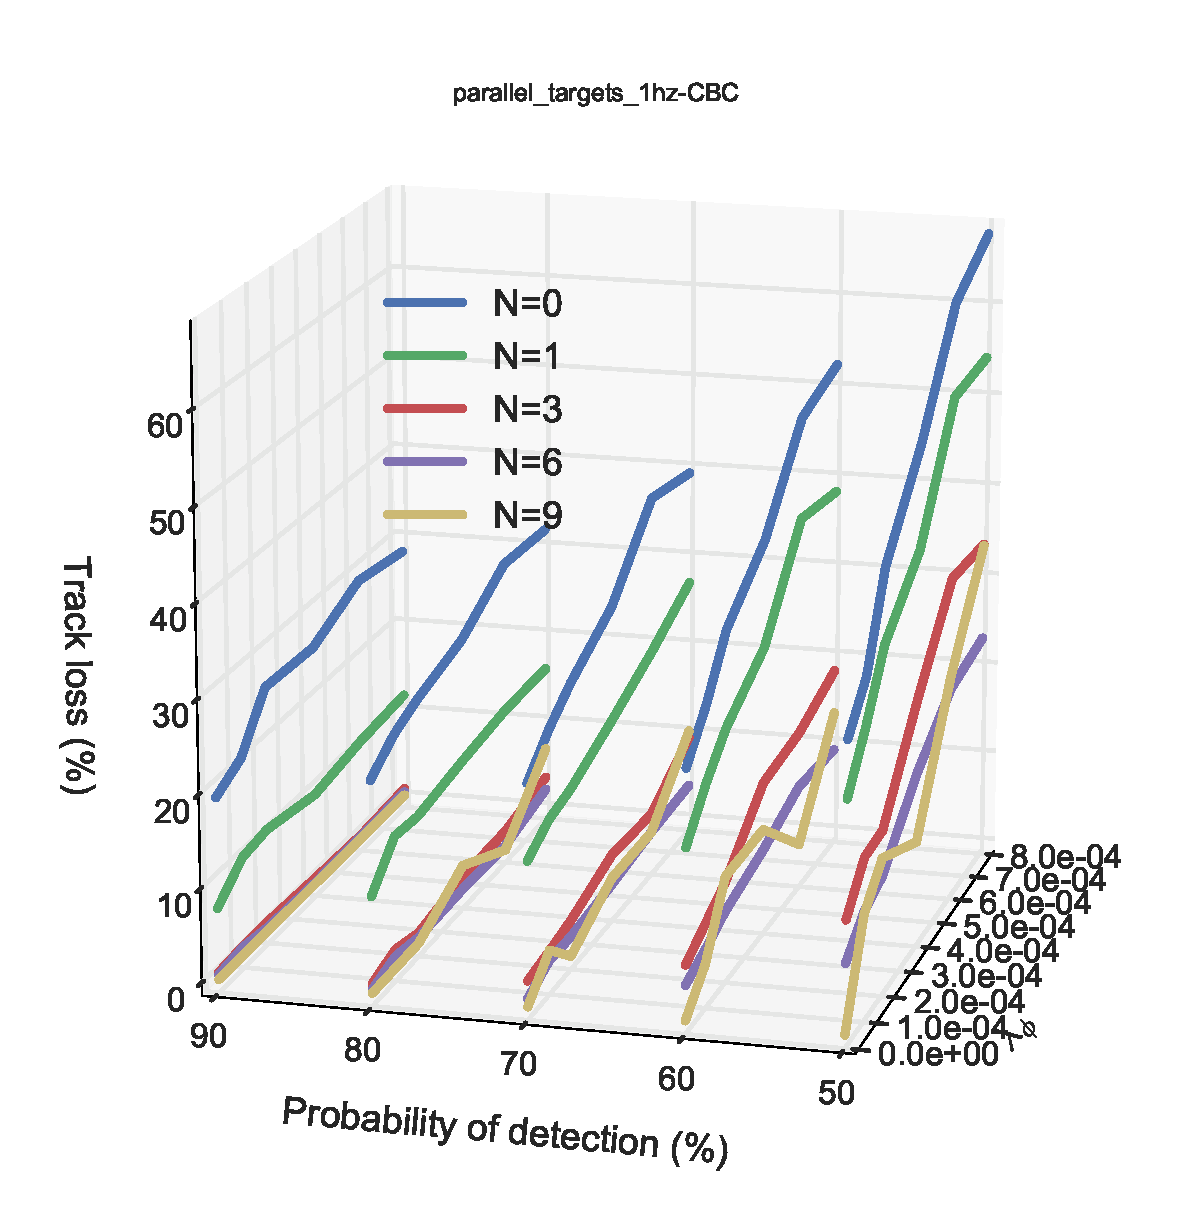
\includegraphics[width=\textwidth]{parallel_targets_1hz-CBC}
        \caption{CBC solver}
    \end{subfigure}
    \begin{subfigure}{0.49\textwidth}
        \centering
        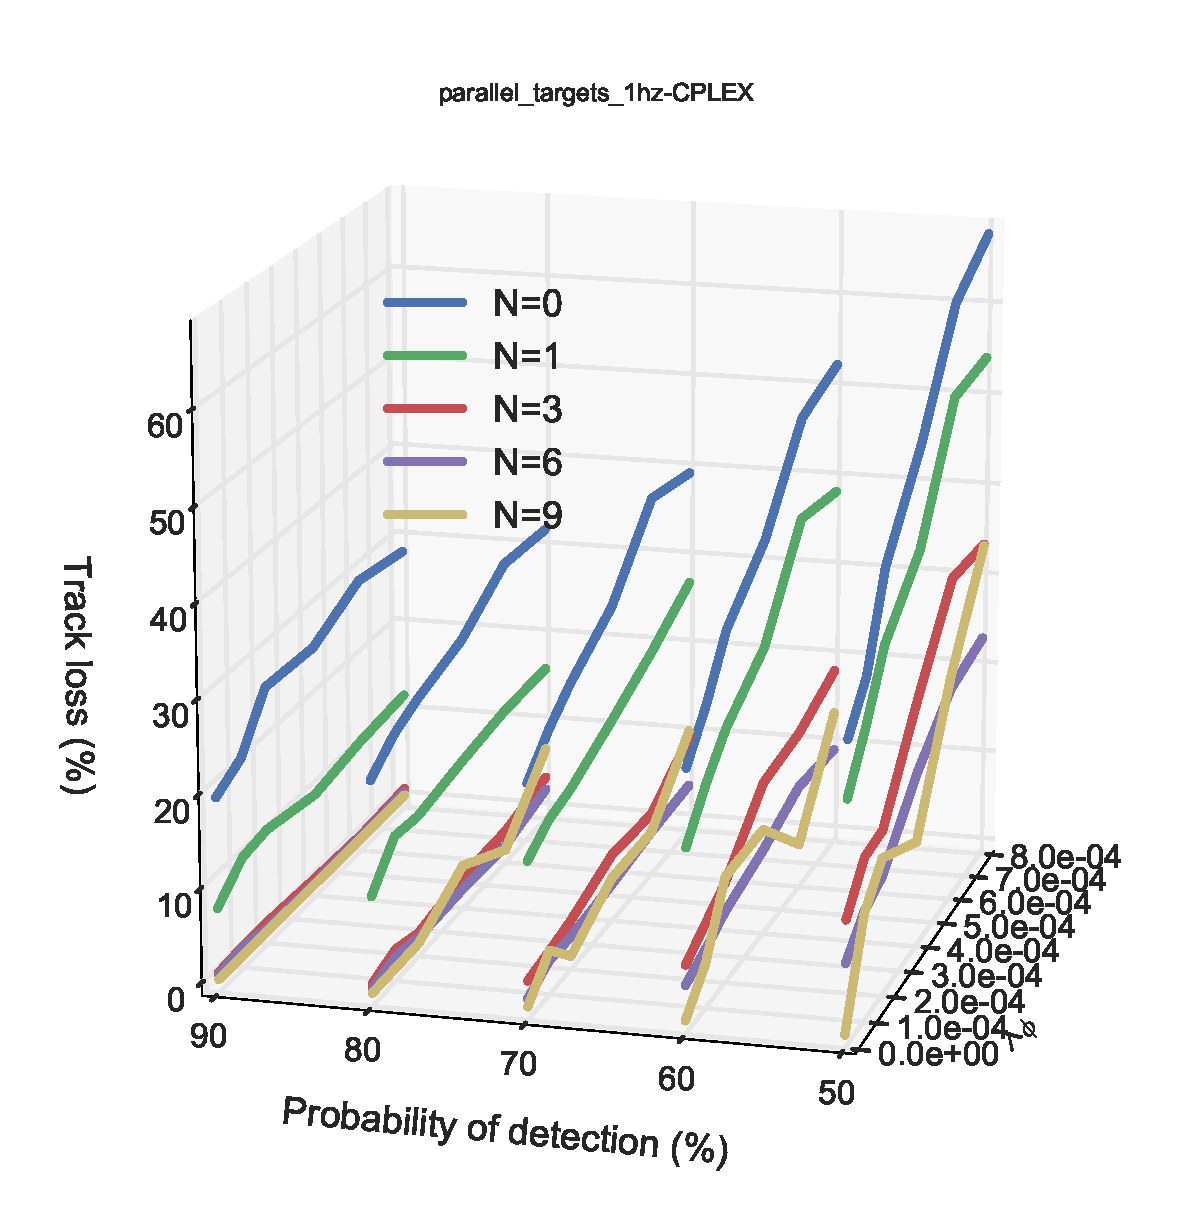
\includegraphics[width=\textwidth]{parallel_targets_1hz-CPLEX}
        \caption{CPLEX solver}
    \end{subfigure}
    \begin{subfigure}{0.49\textwidth}
        \centering
        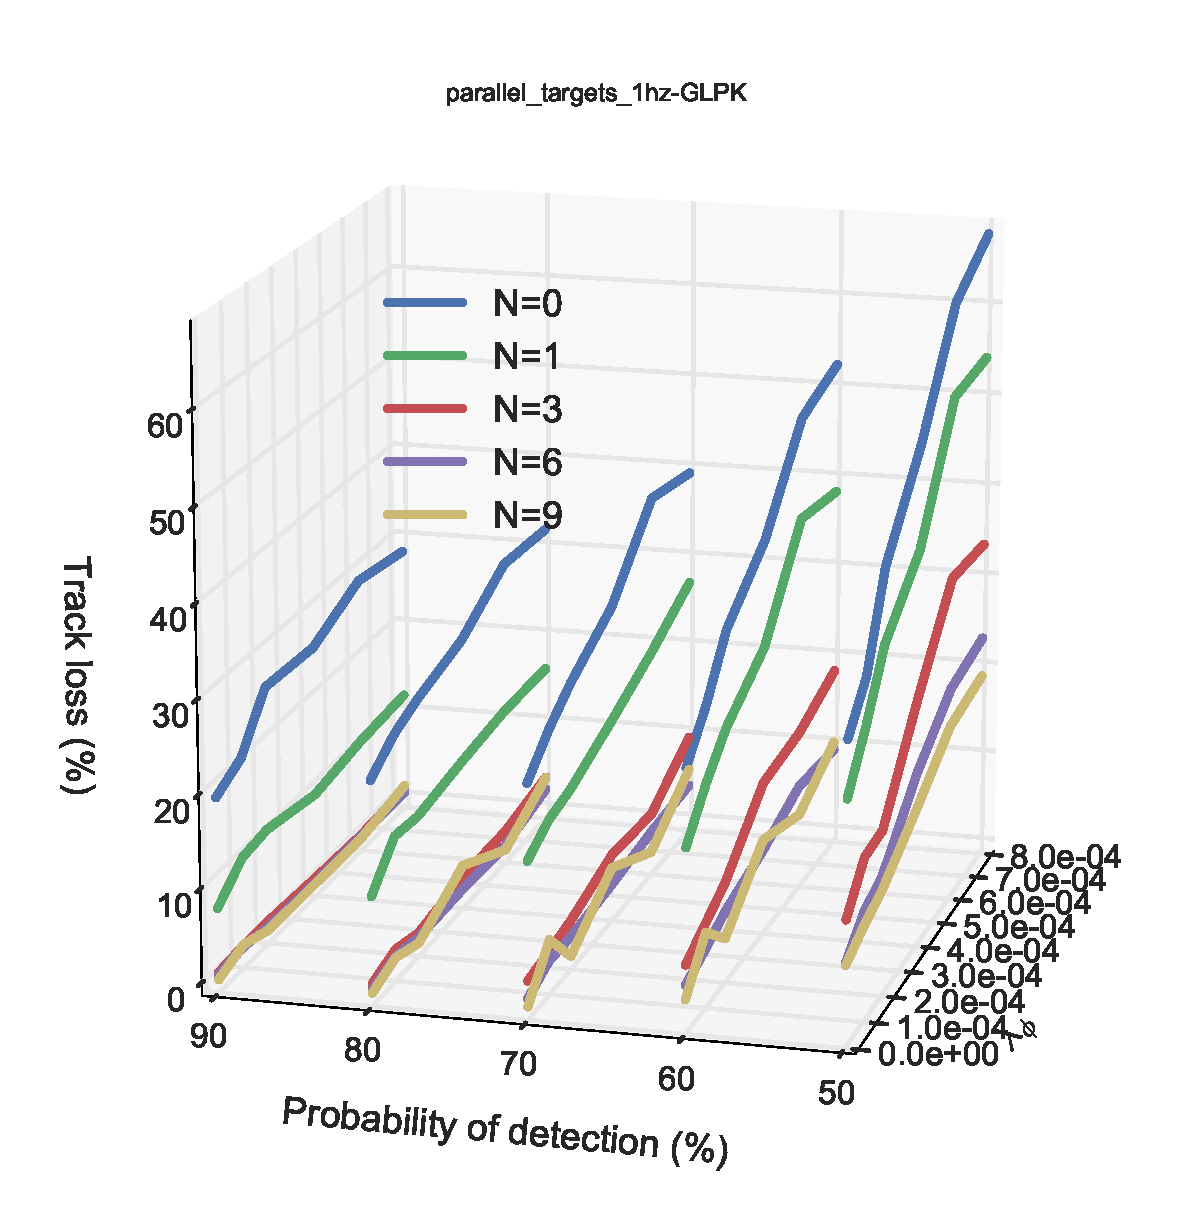
\includegraphics[width=\textwidth]{parallel_targets_1hz-GLPK}
        \caption{GLPK solver}
    \end{subfigure}
    \begin{subfigure}{0.49\textwidth}
        \centering
        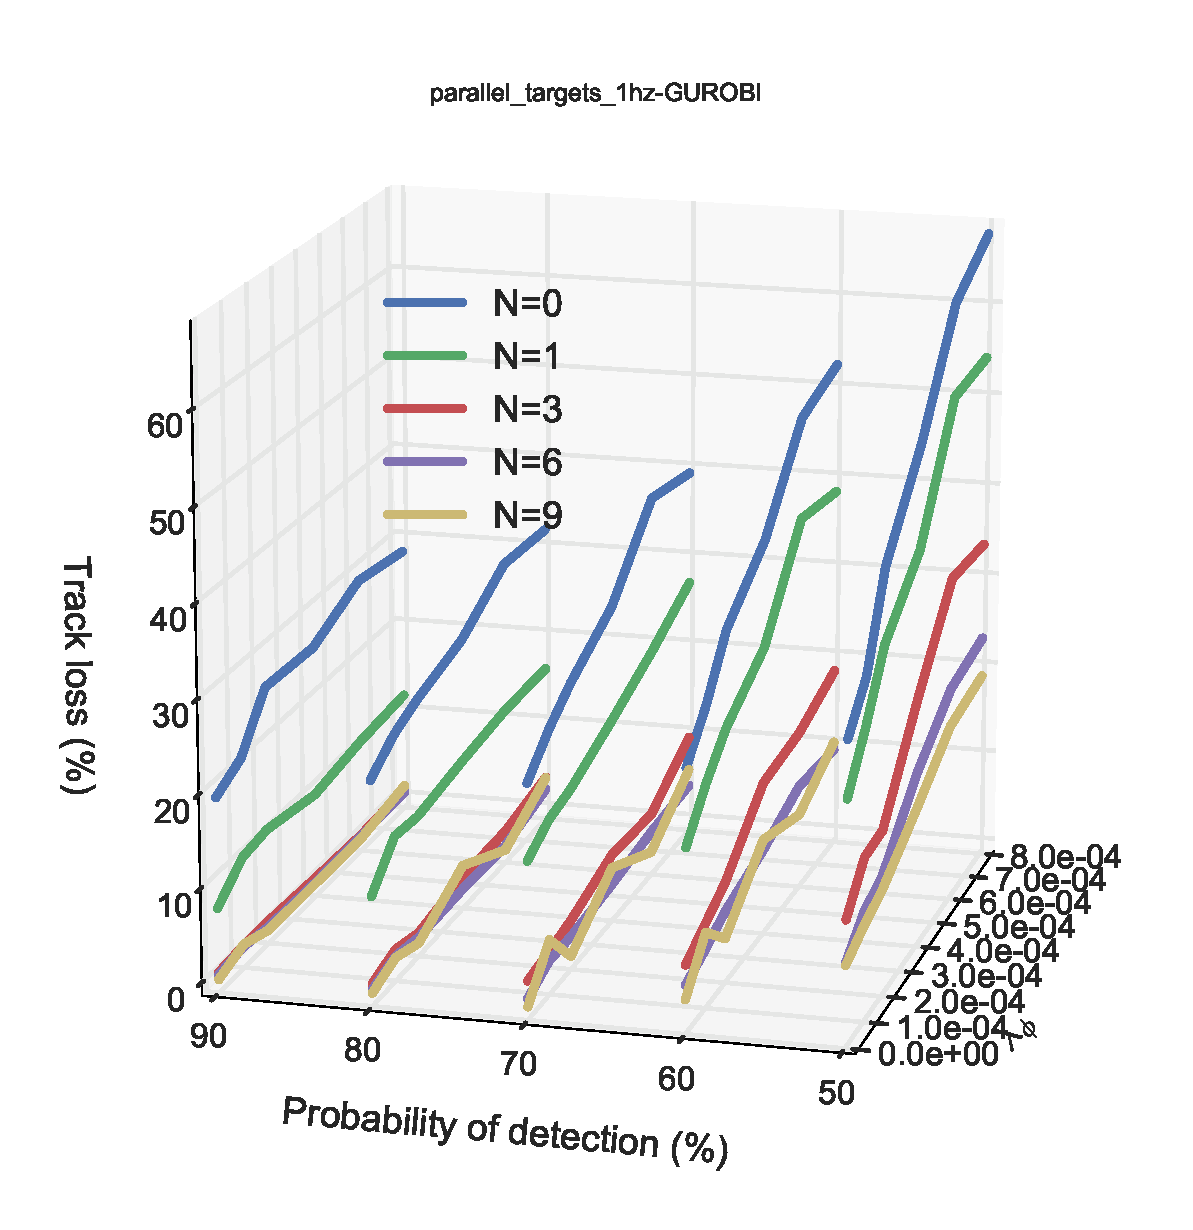
\includegraphics[width=\textwidth]{parallel_targets_1hz-GUROBI}
        \caption{GUROBI solver}
    \end{subfigure}
    \caption{Simulation results for all solvers in scenario 5}
    \label{fig:parallel_targets_1hz}
\end{figure} 
\begin{figure}[H]
    \centering
    \textbf{Scenario 6 - Track performance}\par \medskip
    \begin{subfigure}{0.49\textwidth}
        \centering
        \includegraphics[width=\textwidth]{{parallel_targets_0.5hz-CBC}.pdf}
        \caption{CBC solver}
    \end{subfigure}
    \begin{subfigure}{0.49\textwidth}
        \centering
        \includegraphics[width=\textwidth]{{parallel_targets_0.5hz-CPLEX}.pdf}
        \caption{CPLEX solver}
    \end{subfigure}
    \begin{subfigure}{0.49\textwidth}
        \centering
        \includegraphics[width=\textwidth]{{parallel_targets_0.5hz-GLPK}.pdf}
        \caption{GLPK solver}
    \end{subfigure}
    \begin{subfigure}{0.49\textwidth}
        \centering
        \includegraphics[width=\textwidth]{{parallel_targets_0.5hz-GUROBI}.pdf}
        \caption{GUROBI solver}
    \end{subfigure}
    \caption{Simulation results for all solvers in scenario 6}
    \label{fig:parallel_targets_0.5hz}
\end{figure}